\documentclass[final,11pt]{beamer}
\mode<presentation>{\usetheme{I6pd2}}
\usepackage[english]{babel}
%\usepackage[latin1]{inputenc}
\boldmath
%\usepackage[orientation=landscape,size=custom,height=100,width=115]{beamerposter}
\usepackage[orientation=landscape,size=custom,height=100,width=115,scale=2,debug]{beamerposter}

\usepackage{array,booktabs,tabularx,graphicx}
\usepackage{wrapfig,floatrow}
\newcolumntype{Z}{>{\centering\arraybackslash}X}
\newcommand{\pphantom}{\textcolor{ta3aluminium}}
\let\underdot=\d
\renewcommand{\d}[2]{\frac{d #1}{d #2}}

\listfiles

\title{Data Analysis of an Expansion of the EPA’s RadNet Radiation Dosimetry Protocol}
\author{Joshua Moravec, Adrian Sanabria-Diaz, Jeffery Brittenham, Nathan Brady, Kayla McMahon (Dr. Robert I. Price)} 
\institute[University of Nebraska at Kearney]{Physics Department, University of Nebraska at Kearney, Kearney, Nebraska}
\date[\today]{\today}

\newlength{\columnheight}
\setlength{\columnheight}{32in}


\begin{document}
\begin{frame}
	\begin{columns}
		\begin{column}{.30\textwidth}
			\begin{beamercolorbox}[center,wd=\textwidth]{postercolumn}
				\begin{minipage}[T]{.95\textwidth}
					\parbox[t][\columnheight]{\textwidth}{
						\begin{block}{RadNet}
					\small	The Environmental Protection Agency has a nationwide project called RadNet which ``monitors the nation's air, precipitation, drinking water, and pasteurized milk to track radiation in the environment.'' To monitor the air, stations are deployed around the country. At these stations air is sampled continuously at 60 cubic meters per hour. Detectors on the station monitor beta and gamma radioactivity on the filter. These results are reported the EPA. Every three or four days the filter is taken out and the beta and alpha radioactivity is measured after a period of at least five hours. The results and the filter is then sent to the EPA for further analysis.
						\end{block}
						\begin{block}{Procedure}
						\footnotesize Measuring the activity starts within 15 minutes after the filter is removed from the station. Using a scintillator the activity of both beta and alpha decays are measured in decreasing frequency for five or more hours. After measuring, the data is inputed into a text file and a program is then run to fit the data to a double exponential curve (i.e. $y = Ae^{\lambda_1 x} + Be^{\lambda_2 x}$) Using these values, $\mathcal{R}$ can be found which is then used to give a qualitative amount of activity one breathes.
						\end{block}

						\begin{block}{RADNET Station}
						\begin{center}
						\includegraphics[width=.8\linewidth]{pict1}
						\end{center}
						\end{block}
						\vfill
					}
				\end{minipage}
			\end{beamercolorbox}
		\end{column}

		\begin{column}{.39\textwidth}
			\begin{beamercolorbox}[center,wd=\textwidth]{postercolumn}
				\begin{minipage}[T]{.95\textwidth}
					\parbox[t][\columnheight]{\textwidth}{
						\begin{block}{Finding the Activity}
					\footnotesize 	While the EPA project requires a reading after five hours of the filter, additional readings were instead taken at certain intervals. These intervals were chosen to correspond with the differential equation \[\d{A}{t} = -\lambda A\] where $A$ is the activity. The solution, $A = \left(A_{\text{stop}}\right)e^{-\lambda t}$ shows the alpha or beta activity (or $\d{N}{t}$ where $N$ is the number of particles) after the filter is taken from the monitoring station. We can use the differential equation \[\d{A}{t} = \mathcal{R} - \lambda A\] to model the activity while the filter is still in the station. The $\mathcal{R}$ is the rate of increase of activity due to the station pumping air. The solution, $A = \frac{\mathcal{R}}{\lambda}\left(1-e^{-\lambda t}\right)$, allows us to solve for $\mathcal{R}$: \[\mathcal{R} = \frac{\lambda A_{\text{stop}}}{1-\exp(-\lambda t_{\text{stop}})}\] As $t_{\text{stop}}$ is three or four days, it is sufficiently large enough to say \[\mathcal{R} = \lambda A_{\text{stop}}\] Using this number and the rate of air being pumped, the amount of activity per cubic meter can be approximated for the given time interval.
						\end{block}

						\begin{block}{Example Data Fitting from 15 Aug. 2012}
							%Using the differential equations stated above, the Activity before and after the filter is taken can be extrapolated.  bla hi
							\begin{center}
							\begin{tabularx}{\linewidth}{X X}
							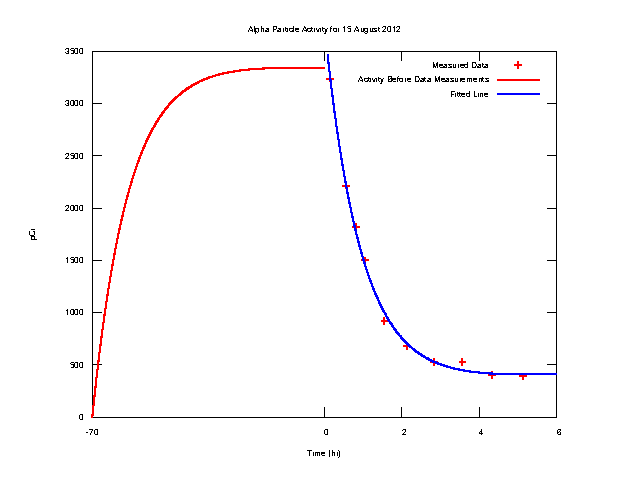
\includegraphics[width=.95\linewidth]{alpha20120815} & 
							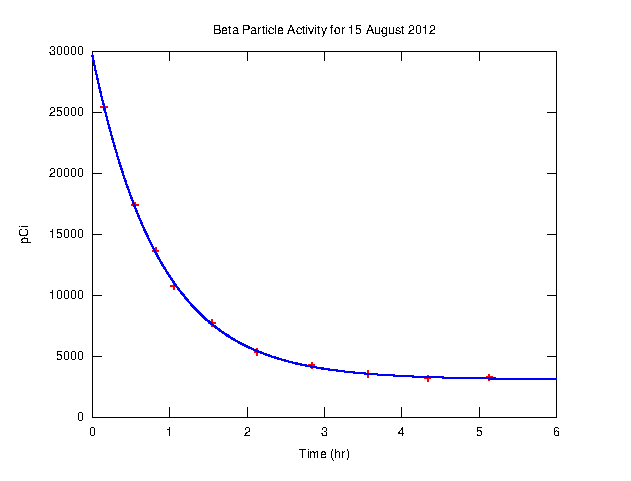
\includegraphics[width=0.95\linewidth]{beta20120815}
							\end{tabularx}
							\end{center}
							\footnotesize These graphs show an example day of data. After the data is measured, the data is fitted to a double exponential $\left(328 e^{0.0353 t} + 3420.69 e^{-1.0679 t}\right)$. Using these values of $A_\text{stop}$ and $\lambda$, the rate during the period the filter is still in the machine is found. For demonstrative purposes, the inferred activity before the filter is measured is shown as the red line. The rates during the period are then collected and are shown in the next graphs.
						\end{block}

						\begin{block}{Acknowledgments}
						\footnotesize Mentor: Dr. Robert Price 

						 EPA RADNET Program: \url{http://www.epa.gov/radnet/index.html}
						\end{block}
					}
				\end{minipage}
			\end{beamercolorbox}
		\end{column}

		\begin{column}{.30\textwidth}
			\begin{beamercolorbox}[center,wd=\textwidth]{postercolumn}
				\begin{minipage}[T]{.95\textwidth}
					\parbox[t][\columnheight]{\textwidth}{
						\begin{block}{Activity over Time}
						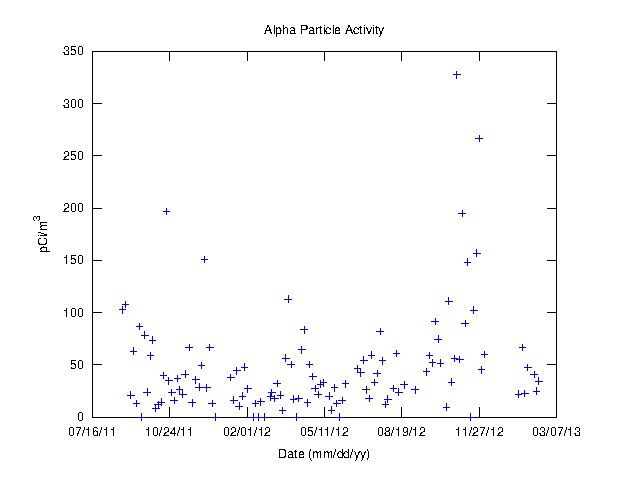
\includegraphics[width=.85\linewidth]{alphaTime}

						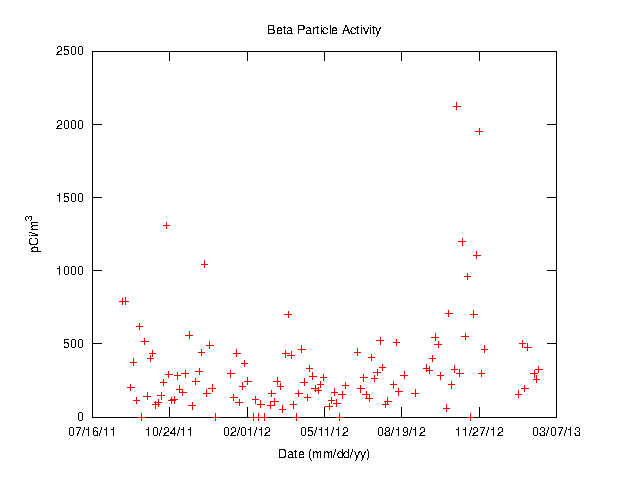
\includegraphics[width=.85\linewidth]{betaTime}
						\end{block}
						\begin{block}{Conclusion}
						\small Although the activity per cubic meter can be found, this data does not allow for analysis of energy. This is due to the fact that the particular isotopes cannot be known using this procedure. However, The analysis can be used to see trends over time in activity amounts of a short and long half life isotopes that may correspond with meteorological or other external events. This is different from the EPA's continuous analysis in that beta as well as alpha radiation is measured. This data, coupled with the assay performed by EPA of the filter may provide a more complete understanding of radioactive activity distribution in America.
						\end{block}
					}
				\end{minipage}
			\end{beamercolorbox}
		\end{column}

	\end{columns}
	\vskip1ex
\end{frame}
\end{document}


